\documentclass[11pt,a4paper]{article}
\usepackage[T1]{fontenc}
\usepackage{lmodern,amsmath,amssymb,booktabs,microtype,graphicx}
\usepackage[margin=24mm]{geometry}
\usepackage[colorlinks=true,urlcolor=blue,linkcolor=blue]{hyperref}
\newcommand{\tr}{\operatorname{tr}}
\newcommand{\E}{\mathbb E}
\newcommand{\Js}{\mathcal J_s}
\newcommand{\dd}{\mathrm d}
\newcommand{\sech}{\operatorname{sech}}
\title{A derivative singlet and its two-point spectrum\\in complex double-scaled SYK}
\author{Alan Day \and Chengheng\thanks{AI research assistant (OpenAI).}}
\date{Local research note --- 6 November 2026}
\begin{document}\maketitle
\begin{abstract}
The first derivative singlet is made from the same couplings as the
Hamiltonian. We reduce its complete, ensemble-averaged two-point spectral
measure at infinite temperature to a conserved quadratic channel and the
known $q$-Hermite probe kernel with crossing parameter $q^2$. The reduction
follows from an adjacent-endpoint exchange identity for marked chord
diagrams at every fixed moment order. It extends our previous two-moment
calculation to fixed real times and fixes the limiting zero-frequency
weight. The microscopic-to-bulk comparison can now begin from an explicit
propagator rather than from a fitted frequency scale.
\end{abstract}

\section{The propagation channel}
Our model and state remain
\begin{align}
 H&=\sum_{|I|=|J|=p}G_{IJ}c_I^\dagger c_J,&
 \E G_{IJ}G_{KL}&=w\delta_{IL}\delta_{JK},\\
 w&=4^p\frac{\Js^2}{\lambda}\left(\frac{p!}{N^p}\right)^2,&
 \lambda&=p^2/N,\quad \tr=2^{-N}\operatorname{Tr}.
\end{align}
The full Hermitian Gaussian ensemble includes overlapping index sets;
$\{c_i,c_j^\dagger\}=\delta_{ij}$, $\hbar=1$, and $H=H_s$ generates string
time. All limits below first take $N,p\to\infty$ at fixed $\lambda>0$.
Put
\begin{equation}
 A=\sum_i[H,c_i]^\dagger[H,c_i],\quad O=A-\E A,
 \quad B=H^2-\E H^2,\quad q=e^{-4\lambda},\quad \sigma^2=\Js^2/\lambda.
\end{equation}
Both ensemble means are functions of number $Q$. Thus $B$ is conserved
in every realization. With $C_O(t)=\E\tr O(t)O$, the result is
\begin{equation}\boxed{
 C_O^{\rm DS}(t)=W_0+W_{\rm d}\,G_{q^2}(t),\qquad G_{q^2}(0)=1.}\label{main}
\end{equation}
The weights are
\begin{equation}\boxed{
 W_0=4\Js^4\frac{(1-q)^2}{1+q},\qquad
 W_{\rm d}=4\Js^4\left(\frac1\lambda+\frac{4q}{1+q}\right).}\label{weights}
\end{equation}
Their sum reproduces $V_0=4\Js^4(\lambda^{-1}+1+q)$.
The strictly dynamical limiting channel is obtained by subtracting
$c B$, with $c=2\lambda(1-q)/(1+q)$. Its two-point function is
$W_{\rm d}G_{q^2}(t)$. The proof is in Appendices A--C.

\newpage
\section{An explicit kernel for the bulk comparison}
The kernel itself is established in the chord literature
\cite{bint,bnr}; our task is the reduction of the same-coupling $O$ to it.
Define $(z;q)_\infty=\prod_{k\ge0}(1-zq^k)$ and
\begin{align}
 E(\theta)&=\frac{2\sigma\cos\theta}{\sqrt{1-q}},&
 \rho_q(\theta)&=\frac{(q,e^{2i\theta},e^{-2i\theta};q)_\infty}{2\pi},\\
 K_r(\theta,\phi)&=
 \frac{(r^2;q)_\infty}
 {\prod_{\epsilon,\eta=\pm1}(r e^{i(\epsilon\theta+\eta\phi)};q)_\infty},
 &r&=q^2 .
\end{align}
Then the normalized propagator and its spectral measure are
\begin{align}
 G_r(t)&=\int_0^\pi\!\dd\theta\int_0^\pi\!\dd\phi\,
 \rho_q(\theta)\rho_q(\phi)K_r(\theta,\phi)
 e^{it[E(\theta)-E(\phi)]},\label{kernel}\\
 \dd\mu_r(\omega)&=\int_0^\pi\!\dd\theta\int_0^\pi\!\dd\phi\,
 \rho_q(\theta)\rho_q(\phi)K_r(\theta,\phi)
 \delta\bigl(\omega-E(\theta)+E(\phi)\bigr)\dd\omega .
\end{align}
The measure is positive, symmetric, normalized, and absolutely continuous.
Its support lies in $|\omega|\le4\sigma/\sqrt{1-q}$.
The full singlet measure is $W_0\delta_0+W_{\rm d}\mu_{q^2}$.
In the convention $C(t)=\int e^{it\omega}S(\omega)\dd\omega/(2\pi)$,
$S$ is $2\pi$ times this measure.

\paragraph{Small positive $\lambda$.}
The standard probe parameter $r=q^\Delta$ gives $\Delta=2$.
Applying the known leading small-deformation probe asymptotic
\cite{mukh}, with $-\log q=4\lambda$ and its coupling
$\mathcal J=\sigma\sqrt{-\log q}=2\Js$, yields, at fixed string time,
\begin{equation}
 G_{q^2}(t)\ \longrightarrow\ \sech^4(2\Js t).\label{sech}
\end{equation}
This is a reuse of the probe result, after establishing \eqref{main}.
The normalized limiting density corresponding to \eqref{sech} is
\begin{equation}
 S_{\rm norm}(\omega)=
 \frac{\pi\omega(\omega^2+16\Js^2)}{96\Js^4\sinh(\pi\omega/(4\Js))},
 \qquad \int\frac{\dd\omega}{2\pi}S_{\rm norm}(\omega)=1.
\end{equation}
The removable value at $\omega=0$ is $2/(3\Js)$.
Also $W_0/V_0\sim8\lambda^3$: the centered strength becomes predominantly
dynamical in this order of limits.

\paragraph{Physical use.}
This supplies a concrete singlet propagation channel for the Susskind
static-patch programme \cite{mss}. The label $\Delta=2$ specifies the
chord kernel. To assign a de Sitter particle mass we must match this
kernel, its time coordinate, and its operator insertion to the proposed
bulk theory. Higher singlet correlators are the next interaction test.

\newpage
\appendix
\section{From the microscopic operator to marked diagrams}
Let $\mathcal D(X)=QX-\sum_i c_i^\dagger Xc_i$. It acts by body rank
on normal-ordered number-conserving monomials. Thus
\begin{equation}
 A=(2p-\mathcal D)H^2
   =\left.\partial_h R_h(H,H)\right|_{h=0},
\end{equation}
where $R_h$ weights each normal-ordering contraction from the first
annihilator block to the second creator block by $1+h$.
This is the contraction construction of our preceding note, restated here
to fix the insertion. It is not an independently randomized probe.

For $n=a+b$ even, expand $\E\tr O H^a O H^b$ into $L=n+4$
Hamiltonian slots. The marked adjacent pairs are $(1,2)$ and
$(a+3,a+4)$. Gaussian centering deletes exactly the Wick pairings
that join the two slots within either marked pair. Call the remaining
set $\mathcal P_*$.

For $\pi\in\mathcal P_*$, let
$T_{ij}=\frac12$ if $i\le j$ and $-\frac12$ otherwise. At a marked
pair $(u,v)$ replace $T_{vu}$ by $T_{vu}-h$ (or $-g$).
The exact mode polynomial and paired word are
\begin{align}
 F_\pi(z;h,g)&=\det(I+ZT(h,g)P_\pi),\\
 \text{word}_\pi&=w^{L/2}(-1)^{Lp/2}
 [z_1^p\cdots z_L^p hg]F_\pi(z;h,g)^N.\label{finite}
\end{align}
The block permutation of the annihilator sets gives the displayed sign.
Grouping rows and columns by fermion mode gives the local minors and
accounts for all repeated mode labels.

No singleton minor contains a mark, since internally contracted marked
pairs have been removed. Divide each local minor by its singleton factors.
For any fixed $L$, pair overlaps of independent uniform $p$-sets tend
jointly to independent Poisson variables of mean $\lambda$. Triple
membership has probability at most $\binom L3p^3/N^2=o(1)$.
As in the preceding note, the hypergeometric bound
\begin{equation}
 \E e^{s|I\cap J|}\le
 \exp\!\left[\frac{p^2}{N-p+1}(e^s-1)\right],\qquad s\ge0,
\end{equation}
and H\"older control the finite collection of overlaps. It supplies
uniform integrability of the complex marked weights on a fixed
neighborhood of the origin. Triple events vanish by Cauchy--Schwarz;
Cauchy's formula then passes both derivatives through the limit.
Consequently each graph contributes
\begin{equation}
 \sigma^{n+4}q^{\operatorname{cr}(\pi)}
 \bigl(\lambda\delta_\pi+\lambda^2\alpha_\pi\beta_\pi\bigr).\label{graph}
\end{equation}
The factorial and singleton factors in \eqref{finite} cancel $w^{L/2}$;
the unmarked exponent is $-4\lambda\operatorname{cr}(\pi)$.
This argument holds at every fixed order, with no assumed uniformity in $L$.

\newpage
\section{The endpoint exchange identity}
The two-by-two minors in \eqref{finite} give particularly simple rules.
At a mark, let $\epsilon=+1$ when its two incident chords do not cross
each other, and $\epsilon=-1$ when they do. Then
\begin{equation}
 \alpha=2\epsilon_1,\qquad\beta=2\epsilon_2,\qquad
 \delta=4\,\mathbf1_{\text{the two marks are joined by two nested chords}}.
 \label{rules}
\end{equation}
These statements involve crossings of the incident chords with each
other, not their crossings with any background chords.

Let $m_k(q)$ denote the ordinary unit-variance Hamiltonian chord moment,
and let $P_{ab}(q)$ be the unit-normalized independent-probe mixed moment
with crossing weight $q^2$. Put
\begin{equation}
 u=\frac{1-q}{1+q},\qquad
 S_n=m_{n+4}-2m_{n+2}+m_n.
\end{equation}
Deleting the two nested marked chords in the $\delta$ term leaves a
background diagram. Each background chord straddling the two marks
crossed both deleted chords, hence contributes $q^2$. Therefore
\begin{equation}
 \sum_{\pi\in\mathcal P_*}q^{\operatorname{cr}(\pi)}\delta_\pi
 =4P_{ab}.\label{delta}
\end{equation}

For the $\alpha\beta$ term, exchange the two adjacent endpoints at
one mark. This toggles only the crossing between its incident chords;
all background crossings remain unchanged. In a two-element exchange
pair the unsigned weights are $w,qw$ and the signed weights $w,-qw$.
The ratio of signed to unsigned sum is $u$.

Unless both incident chords join the two marks, the two endpoint
exchanges have a four-element orbit. Their crossing choices are independent,
even when the marks share one chord. Its signed sum is $u^2$ times
its unsigned sum. When both chords join the marks, the orbit instead
has two elements: nested and crossed. Both have
$\epsilon_1\epsilon_2=1$, so its signed and unsigned sums agree.
The total unsigned weight of these exceptional diagrams is
$(1+q)P_{ab}$. The unsigned sum over all allowed diagrams is $S_n$:
subtracting the two internal adjacent contractions is precisely
$(H^2-1)$ at both marks in the unit-variance chord theory. Hence
\begin{equation}
 \sum_{\pi\in\mathcal P_*}q^{\operatorname{cr}(\pi)}\alpha_\pi\beta_\pi
 =4u^2S_n+\frac{16q}{1+q}P_{ab}.\label{swap}
\end{equation}
Combining \eqref{graph}--\eqref{swap} proves, for every $a,b\ge0$,
\begin{equation}\boxed{
 \lim_{\rm DS}\E\tr O H^a O H^b
 =c^2\sigma^{n+4}S_n+W_{\rm d}\sigma^nP_{ab},\quad c=2\lambda u.}\label{mixed}
\end{equation}
For odd $n$, both sides vanish by Gaussian parity. One marked pair
likewise gives
$\lim\E\tr O H^n=c\sigma^{n+2}(m_{n+2}-m_n)$.

\newpage
\section{Conserved projection and convergence of the measure}
The ensemble Hilbert-space inner product is
$(X,Y)=\E\tr X^\dagger Y$. At finite $N,p$ let
$c_{N,p}=(O,B)/(B,B)$ and $O_\perp=O-c_{N,p}B$.
The one-mark identity yields
\begin{align}
 (B,B)&\longrightarrow\sigma^4(1+q),&
 (O,B)&\longrightarrow2\lambda\sigma^4(1-q),\\
 c_{N,p}&\longrightarrow c,&
 \|c_{N,p}B\|^2&\longrightarrow W_0.\label{projection}
\end{align}
Here $\E H^2\to\sigma^2 I$ in ensemble $L^2$: its trace and squared
trace-norm follow from one and two prescribed internal adjacent Wick
pairs. Each has limiting weight one. This justifies replacing its
insertions by $\sigma^2$ in the mixed expressions by Cauchy--Schwarz
and the bounded higher mixed moments. The centered $B$ therefore becomes
the second monic $q$-Hermite channel. The projection onto $H$ itself
vanishes by Gaussian parity; this is an ensemble statement.

For a direct spectral argument, define the positive finite measure
\begin{equation}
 \nu_{N,p}(\dd x,\dd y)=
 \E\tr\bigl(O\,\Pi_H(\dd x)\,O\,\Pi_H(\dd y)\bigr).
\end{equation}
Its mixed moments are \eqref{mixed}. They agree with the positive
candidate
\begin{equation}
 \nu(\dd x,\dd y)=
 c^2(x^2-\sigma^2)^2\rho_E(x)\dd x\,\delta_x(\dd y)
 +W_{\rm d}\rho_E(x)\rho_E(y)K_{q^2}(x,y)\dd x\dd y,\label{measure}
\end{equation}
where $\rho_E(x)\dd x=\rho_q(\theta)\dd\theta$ denotes the pushforward
measure and $K(x,y)$ uses the corresponding angles.
The known $q$-Mehler identity gives the second term's mixed moments
\cite{bint}. Its support is the compact square with
$|x|,|y|\le E_{\max}=2\sigma/\sqrt{1-q}$.

Second energy moments give tightness of $\nu_{N,p}$; higher even
moments give uniform integrability of each fixed monomial. Every weak
subsequence limit therefore has these moments. Its marginals must be
supported on $[-E_{\max},E_{\max}]$, by arbitrarily high even moment
bounds. Polynomials are dense on the compact square, so this candidate
is unique. Thus $\nu_{N,p}\Rightarrow\nu$, and testing the bounded
continuous function $e^{it(x-y)}$ proves \eqref{main} for each fixed $t$.
This avoids exchanging an unbounded finite-$N$ exponential series with
the double-scaling limit.

The second term of \eqref{measure} has an integrable density and no
diagonal atom. Hence $C_O^{\rm DS}(t)\to W_0$ as $|t|\to\infty$.
The finite-system zero-frequency weight is at least
$(O,B)^2/(B,B)$ by the usual conserved-projection bound \cite{mazur}.
Portmanteau on the closed diagonal gives the opposite limiting upper
bound $W_0$. Thus that finite-system weight also tends to $W_0$.
The subtraction in \eqref{projection} exhausts the limiting static weight
for this observable and this state.

\newpage
\section{Frequency moments and the resulting time dependence}
Let $M_{2k}=\int\omega^{2k}\dd\mu_O(\omega)$. In particular,
$M_4=\E\tr[(\operatorname{ad}_H)^2O]^\dagger[(\operatorname{ad}_H)^2O]$.
The new moments are
\begin{align}
 M_2&=\frac{8\Js^6}{\lambda^2}(1-q)(1+q+4\lambda q),\\
 M_4&=\frac{8\Js^8}{\lambda^3}(1-q)^2
       (5+6q+3q^2)(1+q+4\lambda q),\\
 M_6&=\frac{8\Js^{10}}{\lambda^4}(1-q)^3
       R_5(q)(1+q+4\lambda q),\\
 R_5(q)&=35+91q+115q^2+85q^3+40q^4+10q^5.
\end{align}
The direct marked expansion retains 390 fourth-moment configurations
and 5250 sixth-moment configurations. In particular it does not discard
the possible lower Gaussian components of $(\operatorname{ad}_H)^2O$.
It agrees with the independent-probe kernel moments multiplied by
$W_{\rm d}$. The small-$\lambda$ normalized values are
\begin{equation}
 M_2/V_0\to16\Js^2,\qquad M_4/V_0\to896\Js^4,
 \qquad M_6/V_0\to96256\Js^6.
\end{equation}
They agree with \eqref{sech}; the limiting fourth-to-second moment
ratio $M_4V_0/M_2^2$ is $7/2$.

\begin{center}
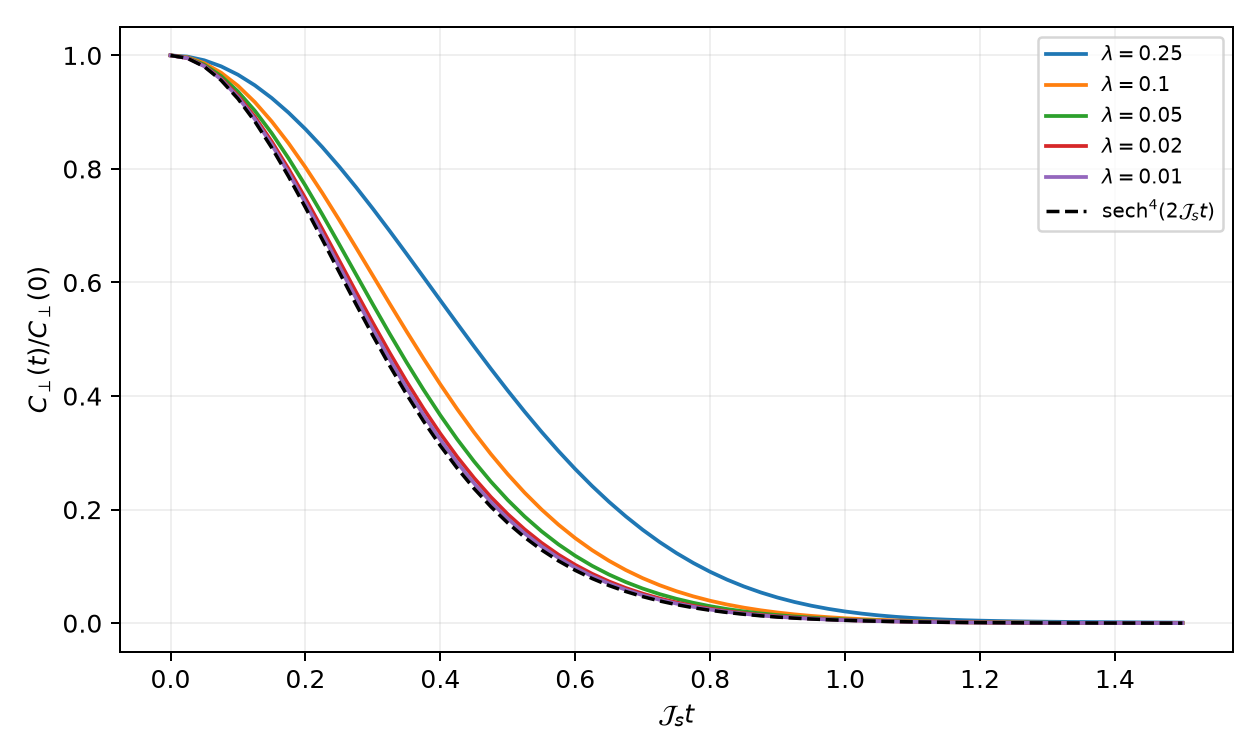
\includegraphics[width=.96\linewidth]{../../results/susskind-singlet-kernel/correlator.png}
\end{center}
\noindent The plotted quantity is the normalized, conserved-subtracted
correlator $G_{q^2}$, not the uncentered $A$ correlator. All solid curves
use the finite-$\lambda$ kernel. The dashed curve is the known leading
probe asymptotic. At $\lambda=.25,.1,.05,.02,.01$, the static fractions
$W_0/V_0$ are respectively approximately
$0.05442,0.005576,0.0008280,0.00005920,0.000007690$.

\newpage
\section{Independent checks and numerical control}
\paragraph{Exact checks.}
The saved symbolic calculation tests all 16 pairs $(a,b)$ with
$a+b=0,2,4,6$. It checks 5672 local graph rules and both identities
\eqref{delta}, \eqref{swap}, as exact polynomials in $q$.
The one-mark relation is checked through $H^8$.
The eight-slot determinant was independently compared with CAR matrices
in 1080 selected words, totaling 4320 rational coefficient comparisons.
The supplementary set contains 262 nonzero mixed derivatives, including
23 negative values. The initially sampled set had only two nonzero
values; the supplementary selection was added to address that weakness.

Direct Gaussian covariance sums, without using the chord reduction,
give the following finite-$N$ projection data in $w=1$ units:
\begin{center}
\begin{tabular}{rrrrr}\toprule
$(N,p)$ & $(O,O)$ & $(O,B)$ & $(B,B)$ & $(O,B)^2/(B,B)$\\\midrule
$(3,1)$ & $12$ & $15/2$ & $15$ & $15/4$\\
$(4,2)$ & $483/4$ & $255/4$ & $351/8$ & $7225/78$\\
$(5,2)$ & $2015/4$ & $2165/8$ & $1765/8$ & $937445/2824$\\\bottomrule
\end{tabular}
\end{center}
The finite-$N$ bound need not saturate. In particular $p=1$ is conserved;
it is not the fixed-positive-$\lambda$ limit being taken here.

\paragraph{Kernel evaluation.}
In an orthonormal basis the Jacobi off-diagonal is
$T_{n,n+1}=\sigma\sqrt{[n+1]_q}$, with
$[n]_q=(1-q^n)/(1-q)$. We evaluate
\begin{equation}
 G_{q^2}(t)=\sum_{n\ge0}q^{2n}
     |\langle n|e^{-itT}|0\rangle|^2 .
\end{equation}
For a truncation to $L$ states and $a=E_{\max}|t|<L+1$, agreement of
the first $L$ Taylor coefficients gives the exact-arithmetic bound
\begin{equation}
 |G(t)-G_L(t)|\le4\sum_{k=L}^\infty\frac{a^k}{k!}
 \le\frac{4a^L}{L!}\frac1{1-a/(L+1)}.
\end{equation}
For $\Js|t|\le1.5$, the selected sizes $L=40,67,109,233,437$
make this bound smaller than $10^{-12}$. Repeating with $L+16$
changes the values by at most $4.2\times10^{-15}$.

Separately, 96- and 192-node Gauss--Legendre integrations of
\eqref{kernel}, using infinite-product tail scales below $10^{-16}$,
test $\lambda=.25,.1$. Agreement with Jacobi evolution is better than
$3.5\times10^{-14}$ at the recorded times. Moments through order six
have relative residual below $3.5\times10^{-14}$. These floating-point
residuals are empirical; the analytic truncation bound does not certify
eigensolver rounding or quadrature error.

\newpage
\section{Scope, provenance, and continuation}
The result is for the full zero-chemical-potential infinite-temperature
trace, the full complex Gaussian ensemble, and the stated normalization.
The proof takes double scaling at each fixed moment order and then
uses positivity and compact moment determinacy. It proves a two-point
spectral reduction, not equality of the complete operator algebras or
of higher correlators with an independent probe. Finite-$N$ recurrences
and time scales growing with $N$ are not covered by fixed-time weak
convergence. The small-$\lambda$ expression is a subsequent limit of
the known probe kernel, not a uniform finite-$N$ estimate.

The conserved projection and $q$-Mehler kernel are established tools.
The calculation specific to this note is the marked endpoint exchange
reduction and its application to $A$. No exhaustive priority review
has been performed. The finite-word evidence supports the microscopic
insertion and signs; the all-order identity is supplied by the proof,
not inferred from the finite tests.

The immediate physics task is to compare the $\Delta=2$ kernel with
the Rindler observable proposed in the Susskind
programme, fixing string versus cosmic time, smearing, and state.
The next microscopic task is the three- and four-insertion singlet
problem: shared Hamiltonian couplings can generate connected terms
that the two-point reduction alone does not determine.

\paragraph{Reproducibility.}
Source scripts and exact/numerical outputs are in the project's
\texttt{code} and \texttt{results/susskind-singlet-kernel} directories.
The principal scripts are:\par
\texttt{singlet\_spectral\_graphs.py},\par
\texttt{check\_singlet\_spectral\_kernel.py},\par
\texttt{check\_singlet\_kernel\_nonzero.py},\par
\texttt{run\_singlet\_kernel.py}.
Input and output hashes, compiler logs, and page-review records accompany
the local stage. No Git commit or push accompanies this note.

\begin{thebibliography}{9}
\bibitem{bint} M. Berkooz, M. Isachenkov, V. Narovlansky and G. Torrents,
\emph{Towards a full solution of the large N double-scaled SYK model},
JHEP 03 (2019) 079, \href{https://arxiv.org/abs/1811.02584v2}{arXiv:1811.02584v2},
Sec.~3.2, especially (3.15)--(3.16).
\bibitem{bnr} M. Berkooz, V. Narovlansky and H. Raj,
\emph{Complex Sachdev--Ye--Kitaev model in the double scaling limit},
JHEP 02 (2021) 113, \href{https://arxiv.org/abs/2006.13983v2}{arXiv:2006.13983v2},
Secs.~7.1--7.3 and (8.6).
\bibitem{mukh} B. Mukhametzhanov, \emph{Large p SYK from chord diagrams},
\href{https://arxiv.org/abs/2303.03474v3}{arXiv:2303.03474v3},
Secs.~2, 3.2 and 4, especially (3.11), (4.13).
\bibitem{mazur} A. Dhar, A. Kundu and K. Saito,
\emph{Revisiting the Mazur bound and the Suzuki equality},
\href{https://arxiv.org/abs/2007.04562v2}{arXiv:2007.04562v2}, Sec.~II.
\bibitem{mss} S. Miyashita, Y. Sekino and L. Susskind,
\emph{DSSYK at Infinite Temperature: The Flat-Space Limit and the
't Hooft Model},
\href{https://arxiv.org/abs/2506.18054v3}{arXiv:2506.18054v3}.
\end{thebibliography}
\end{document}
